\documentclass[11pt]{article}
\usepackage{fontspec}
\setmainfont{Libertinus Serif}
\usepackage[margin=2cm]{geometry}
\usepackage{tikz-uml}
\usepackage{graphicx}

\begin{document}
\section*{MVC-Muster}
Bei der Realisierung von Benutzeroberflächen kommt das MVC-Muster zum Einsatz.
\begin{itemize}
\item \textbf{Modell}, der Kern des Systems (Objekte, ihre Daten, Methoden und Beziehungen)
\item \textbf{View} (Sicht auf die Daten)
\item \textbf{Controller} (Verarbeitung von Benutzereingaben, Synchronisieren von Modell und View).
\end{itemize}
Im Beispiel soll eine Temperaturanzeige realisiert werden. Die angezeigte Temperatur kann durch zwei Buttons erhöht und erniedrigt werden.
\begin{center}
\includegraphics[width=3cm]{images/gui}
\end{center}
Ein Temperatur-Objekt wird im Fenster zur Ansicht gebracht. Ein Controller-Objekt verarbeitet die Interaktion eines Benutzers mit den Buttons. Dabei passt es den Wert des Temperatur-Objekts an und informiert das Fenster, dass die Darstellung aktualisiert werden muss. Es kommen die folgenden Klassen zum Einsatz:
\begin{center}
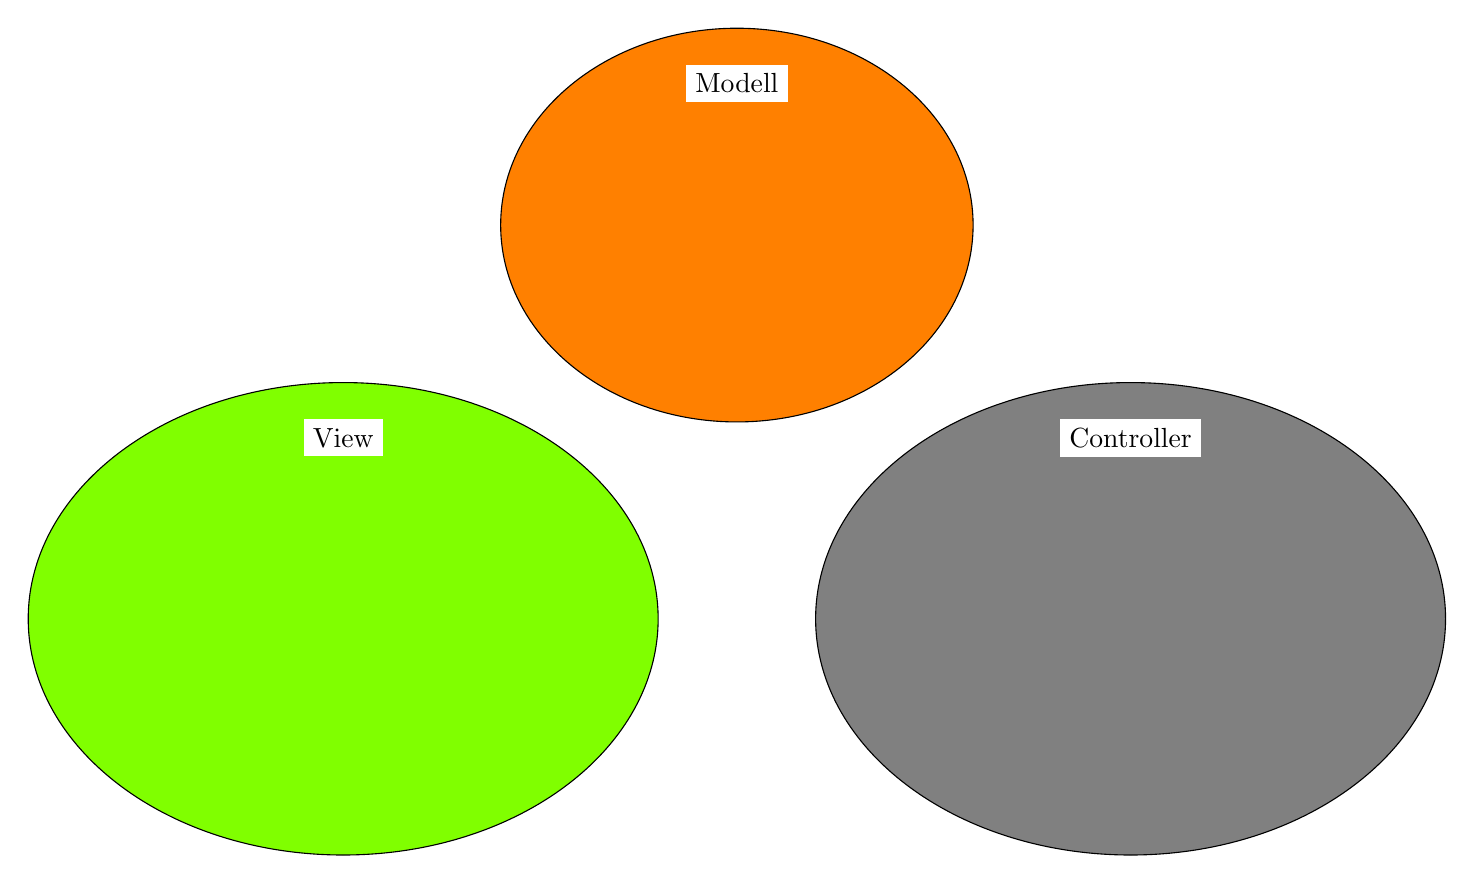
\begin{tikzpicture}[scale=1]
\draw[fill=red!50!yellow](0,0) ellipse (3cm and 2.5cm);\node[fill=white] at (0,1.8){Modell};
\umlclass{Temperatur}{value: double}{up():\\down():}
\draw[fill=green!50!yellow](-5,-5) ellipse (4cm and 3cm);\node[fill=white] at (-5,-2.7){View};
\umlclass[x=-5, y=-5]{TemperatureView}{value: Temperature\\controller: TemperatureController\\lTemperatur: JLabel\\bUp: JButton\\bDown: JButton}{update():}
\draw[fill=blue!50!yellow](5,-5) ellipse (4cm and 3cm);\node[fill=white] at (5,-2.7){Controller};
\umlclass[x=5, y=-5]{TemperatureController}{value: Temperature\\view: TemperatureView} {addView(TemperatureView):\\actionperformed(ActionEvent):}
\umlassoc[->]{TemperatureView}{Temperatur}
\umlassoc[->]{TemperatureController}{Temperatur}
\umlassoc[<->]{TemperatureView}{TemperatureController}
\end{tikzpicture}
\end{center}
\end{document}